
In this section, we report the automatic and human preference evaluation of the Chat Model. 
We use greedy decoding to generate responses. For the automatic evaluation benchmarks, we extract answers from the model's generated outputs and calculate accuracy. During the evaluation process, we observed that different prompts have varying influence on  results. Therefore, for the same set of questions, we use identical prompts to evaluate all models, aiming to ensure as fair and unbiased results as possible.

% 
\begin{table}
  \centering
  \begin{tabular}{lccccc}
\toprule
Model & Size & Avg & SQUAD & QUAC & BoolQ\\
\midrule
GPT-3.5 & - & - & - & - & 87.2 \\
GPT-4 & - & - & - & - & 90.6 \\
\gmidrule
Falcon & 180B & - & 50.8 & - & 86.8 \\
\gmidrule
\multirow{2}{*}{Qwen} & 7B & 59.5 & 74.1 & 36.7 & 67.8\\
 & 14B & 72.5 & 84.2 & 47.8 & 85.5\\
 \gmidrule
Baichuan 2 & 13B & 62.4 & 74.0 & 39.7 & 73.6\\
% \midrule
% Open-L\textsmaller{LaMA} v2 & 7B & & & & & &  \\
\gmidrule
\multirow{3}{*}{L\textsmaller{LaMA} 2} & 7B & 61.3 & 67.2 & 39.4 & 77.4\\
& 34B & 68.9 & 78.8 & 44.3 & 83.7   \\
& 70B & 72.3 & 82.6 & \textbf{49.4} & 85.0 \\
\gmidrule
Mistral & 7B & - & - & - & 83.5\\
\gmidrule
InternLM & 20B & - & - & - & 87.5 \\
\gmidrule
Skywork & 7B & 64.9 & 70.9 & 41.0 & 82.9 \\
\gmidrule
\multirow{2}{*}{Yi}
& 6B & 68.7 & 89.0 & 40.9 & 76.2\\
& 34B & \textbf{76.5} & \textbf{92.5} & 48.6 & \textbf{88.3}\\
\bottomrule

  \end{tabular}
   \caption{Comparison to open-source models on reading comprehension, (SQUAD and QUAC).
   % \alex{what kind of prompt did we use? do we test the numbers of all these models on our own, or we copy the number from their papers?}
   }
  \label{tab:reading_comprehension}
\end{table}


\subsubsection{Automatic Evaluations}

% We employed some of the identical evaluation datasets as those used for the base model to assess the general capabilities of our model in Sec. \ref{sec:main results}.

For automatic evaluation, we use the same benchmarks as is for the base model, detailed in Sec. \ref{sec:main results}.
We use both zero-shot and few-shot methods but generally, zero-shot is more suitable for chat models. Our evaluation involves generating responses while following instructions explicitly or implicitly (such as the format in the few-shot examples). We then isolate relevant answers from the generated text. Unlike the base model, for the zero-shot evaluations on the GSM8K and BBH datasets, we employ the Chain-of-Thought (CoT) approach to guide the model in deliberation before reaching an answer.


The results shown in Tab. \ref{tab:chat_models} demonstrate the effectiveness of our chat models in understanding human instructions and generating appropriate instruction-following responses. 
We particularly highlight the 4-bit quantization results, as 4-bit quantization substantially reduces the memory requirement while the model performance nearly does not drop. 
This observation serve as the foundation of serving the model on consumer-grade devices. 

% The results indicate that the Yi-34B-Chat model exhibits commendable performance on evaluation sets encompassing Chinese-English knowledge-based, mathematical, and reasoning categories.


In line with Goodhart's principle, when a measurement metric becomes the target of our pursuit, it ceases to serve as a reliable standard of assessment. Consequently, the outcomes of our evaluations on benchmarks are exclusively employed for ensuring that our alignment training does not detrimentally impact the foundational knowledge and capabilities of the base model. We do not engage in targeted optimization of our chat model with the objective of enhancing benchmark performance.


To further evaluate the generalizability of our model's capabilities, we conducted assessments of its mathematical computation proficiency by subjecting it to the 2023 Hungarian high school mathematics final exam questions, first proposed by the xAI Grok team then reproduced by~\citet{testing_language_models_on_a_held_out_high_school_national_finals_exam}. This evaluation was undertaken with the aim of determining whether our model exhibited signs of overfitting to training datasets that are mathematically oriented.
The results in Fig.~\ref{fig:hungarian_national_hs_finals_exam} show that Yi-34B-Chat performs inspiringly on both the GSM8K and the Hungarian mathematics exam. However, note that Yi-6B-Chat does not exhibit strong mathematical capabilities (on both GSM8K and the Hungarian mathematics exam). We speculate that smaller models may require more data to activate their corresponding abilities during the SFT stage.


\begin{table*}[t!]
\centering
% \scalebox{0.75}{
\setlength\tabcolsep{2pt}
\resizebox{\textwidth}{!}{
\begin{tabular}{@{}l c c c c c c c c c c c@{}}
\toprule
\multicolumn{1}{l}{\multirow{2}{*}{\textbf{Model}}}  & \multicolumn{1}{c}{\multirow{2}{*}{\textbf{Size}}} & \multicolumn{1}{c}{\multirow{2}{*}{\textbf{MMLU}}}   & \multicolumn{1}{c}{\multirow{2}{*}{\textbf{CMMLU}}} & \multicolumn{1}{c}{\multirow{2}{*}{\textbf{C-Eval(val)}}} & \multicolumn{1}{c}{\multirow{2}{*}{\textbf{TruthfulQA}}} & \multicolumn{1}{c}{\multirow{2}{*}{\textbf{BBH}}} & \multicolumn{1}{c}{\multirow{2}{*}{\textbf{GSM8K}}} \\ 

\multicolumn{1}{c}{} & \multicolumn{1}{c}{} & \multicolumn{1}{c}{} & \multicolumn{1}{c}{}    & \multicolumn{1}{c}{}  & \multicolumn{1}{c}{} & \multicolumn{1}{c}{} &  \multicolumn{1}{c}{} &  \multicolumn{1}{c}{} \\

\multicolumn{1}{c}{} & \multicolumn{1}{c}{} & \multicolumn{1}{c}{\textbf{0-shot / 5-shot}}  & \multicolumn{1}{c}{\textbf{0-shot / 5-shot}} & \multicolumn{1}{c}{\textbf{0-shot / 5-shot}} &  \multicolumn{1}{c}{\textbf{0-shot}} &  \multicolumn{1}{c}{\textbf{0-shot / 3-shot}} & \multicolumn{1}{c}{\textbf{0-shot / 4-shot}}  \\

\midrule

LLaMA2-Chat
& 13B & 50.9 / 47.3 & 27.5 / 35.1 & 27.9 / 35.9 & 36.8 & 32.9 / 58.2 & 36.9 / 2.7 \\
& 70B & 59.4 / 59.9 & 36.1 / 41.0 & 35.0 / 41.3 & 54.0  & 42.4 / 58.5 & 47.1 / 58.7 \\
\gmidrule
Baichuan2-Chat
& 13B & 55.1 / 50.1 & 58.6 / 59.5 & 56.0 / 54.8 & 49.0 & 38.8 / 47.2 & 45.7 / 23.3 \\
\gmidrule
Qwen-Chat
& 14B & 64.0 / 65.0 & 67.7 / 70.6 & 66.1 / 70.1 & 52.5 & 49.7 / 55.0 & 59.5 / 61.2 \\
\gmidrule
InternLM-Chat
& 20B & 55.6 / 57.4 & 53.6 / 53.8 & 51.2 / 53.6 & 51.8 & 42.4 / 36.7 & 15.7 / 43.4 \\
\gmidrule
AquilaChat2
& 34B & 65.2 / 66.7 & 67.5 / 70.0 & \textbf{83.0} / \textbf{89.4} & \textbf{64.3} & 20.1 / 34.3 & 11.5 / 48.5 \\
\gmidrule
Yi-Chat
& 6B & 58.2 / 61.0 & 69.4 / 74.7 & 68.8 / 74.2 & 50.6 & 39.7 / 47.2 & 38.4 / 44.9 \\
Yi-Chat-8bits(GPTQ)
& 6B & 58.3 / 61.0 & 69.2 / 74.7 & 69.2 / 73.9 & 49.9 & 40.4 / 47.3 & 39.4 / 44.9 \\
Yi-Chat-4bits(AWQ)
& 6B & 56.8 / 59.9 & 67.7 / 73.3 & 67.5 / 72.3 & 50.3 & 37.7 / 43.6 & 35.7 / 38.4 \\
\gmidrule
Yi-Chat
& 34B & \textbf{67.6} / 73.5 & \textbf{79.1} / \textbf{81.3} & 77.0 / 78.5 & 62.4 & 51.4 / \textbf{71.7} & \textbf{71.7} / \textbf{76.0} \\
Yi-Chat-8bits(GPTQ)
& 34B & 66.2 / \textbf{73.7} & 79.1 / 81.2 & 76.8 / 79.0 & 61.8 & \textbf{52.1} / 71.0 & 70.7 / 75.7 \\
Yi-Chat-4bits(AWQ)
& 34B & 65.8 / 72.4 & 78.2 / 80.5 & 75.7 / 77.3 & 61.8 & 48.3 / 69.4 & 70.5 / 74.0 \\

\bottomrule

\end{tabular}
}
\caption{Overall performance on automatic benchmarks compared to open-source chat models. We highlight the 4-bit quantization results, as 4-bit quantization substantially reduces the memory requirement while the model performance nearly does not drop. 
This observation serve as the foundation of serving the model on consumer-grade devices, e.g., RTX4090.
% \yz{Only keep one decimal. I also added the resize command to avoid table overflow.}
}
\label{tab:chat_models}
\end{table*}


\begin{figure}
  \centering
  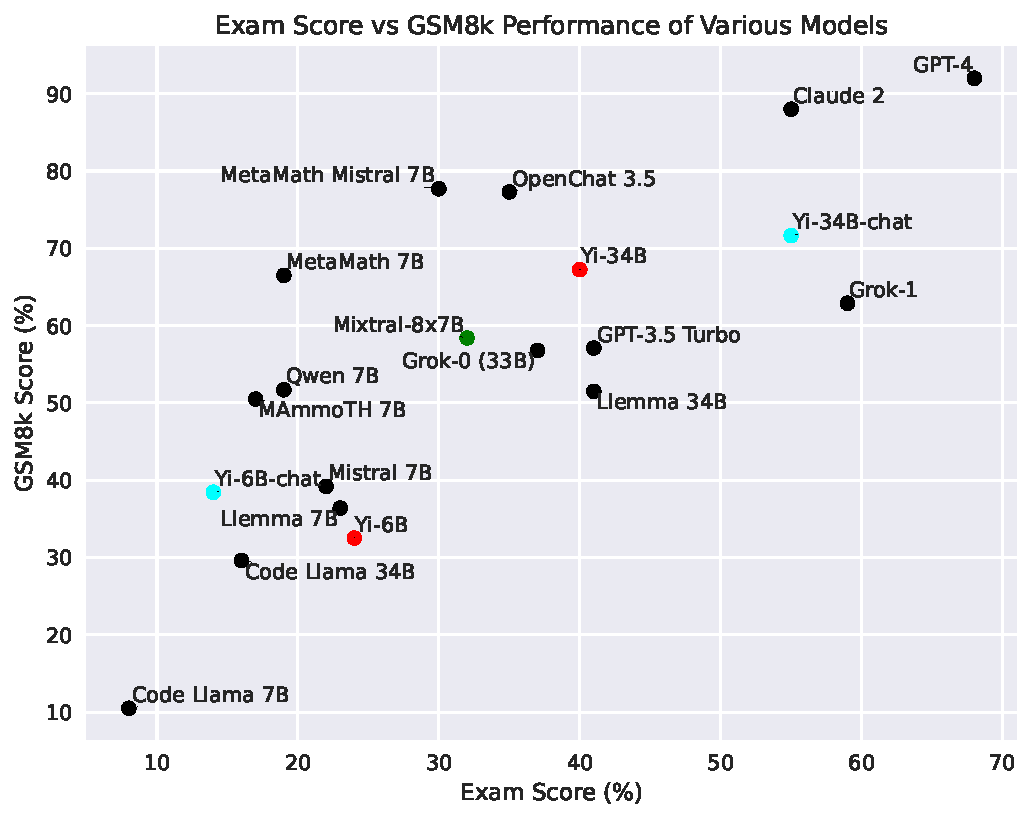
\includegraphics[scale=0.65]{images/hungarian_national_hs_finals_exam.pdf}
  \caption{Yi's result of Hungarian mathematics exam. 
  % \yz{save as a pdf, use ``times new roman'' font when plotting.}
  } 
  \label{fig:hungarian_national_hs_finals_exam}
\end{figure}


\subsubsection{Human Evaluations}

% Our goal is to train an AI assistant that is both helpful and harmless. Consequently, 

In this section we conducted an assessment of the model's conversational abilities, considering aspects to ensure its effectiveness and safety. We have compiled a collection of open-source evaluation datasets from the community, such as alpaca-eval\cite{dubois2023alpacafarm}, Belle-eval~\citep{belle2023exploring}, and MT-bench\cite{zheng2023judging}. Additionally, we have established our own helpful and harmless evaluation dataset by gathering and constructing data of varying difficulty levels, for the purpose of comprehensively assessing the conversational abilities of chat models.

However, whether it is a public evaluation set or a self-built evaluation set, the evaluation results are strongly influenced by the assessment criteria and the design of the prompt. Our internal evaluation results may be unfair to other models, making it difficult to accurately represent the true capability level of our model.
Therefore, here we only present external evaluation results to demonstrate the current conversational abilities of our chat model.
We consider: 
(1). AlapcaEval\footnote{https://tatsu-lab.github.io/alpaca\_eval/}~\citep{alpaca_eval}, which is designed to assess the English conversation capabilities of models by comparing the responses of a specified model to reference replies from Davinci003~\citep{dubois2023alpacafarm} in order to calculate a win-rate;
(2). LMSys\footnote{https://huggingface.co/spaces/lmsys/chatbot-arena-leaderboard}~\citep{zheng2023judging} Chatbot Arena, which showcases the responses of different models through a dialogue platform, then asks users to make selections based on their preferences, then computes the Elo score; (3). SuperClue\footnote{https://www.superclueai.com/}, on the other hand, is a leaderboard aimed at comprehensively evaluating the Chinese language capabilities of models.


\begin{table*}[t!]
\centering
\scalebox{0.9}{
\begin{tabular}{l c c c c c c c c c c c}

\toprule
% \multicolumn{1}{l}{\multirow{1}{*}{\textbf{Model}}}  & \multicolumn{1}{c}{\multirow{1}{*}{\textbf{Size}}} & \multicolumn{1}{c}{\multirow{1}{*}{\textbf{AlpacaEval}}}   & \multicolumn{1}{c}{\multirow{1}{*}{\textbf{lmsys}}} & \multicolumn{1}{c}{\multirow{1}{*}{\textbf{SuperClue}}} \\ 
\bf Model & \bf Size & \bf AlpacaEval & \bf LMSys Chatbot Arena & \bf SuperClue \\ 

% \multicolumn{1}{c}{} & \multicolumn{1}{c}{} & \multicolumn{1}{c}{} & \multicolumn{1}{c}{}    & \multicolumn{1}{c}{}  \\

% \multicolumn{1}{c}{} & \multicolumn{1}{c}{} & \multicolumn{1}{c}{win-rate (\%)}  & \multicolumn{1}{c}{ChatbotArena ELO} & \multicolumn{1}{c}{score} \\

\midrule

GPT-4-Turbo & - &  \textbf{97.7} & \textbf{1243} & \textbf{89.79} \\

% \midrule

GPT-3.5-Turbo & - &  89.37 & 1117 & 59.39 \\

% \midrule

LLaMA2-Chat & 70B &  92.66 & 1077 & - \\

% \midrule

Yi-Chat & 34B &  94.08 & 1110 & 71.87 \\

\bottomrule


\end{tabular}
}
\caption{Human evaluation comparison with other open-source chat models.}
\label{tab:human_evaluation}
\end{table*}


Tab. \ref{tab:human_evaluation} presents the performance results of Yi-34B-Chat in the three third-party evaluations we consider, with the cutoff date for the results being December 21, 2023. The data demonstrates that, although there is still a gap compared to GPT-4, our model exhibits proficient bilingual (Chinese and English) dialogue capabilities and aligns well with user preferences. Additional comparative results of various models are accessible for review on the official website.

\begin{figure}
	\begin{center}
		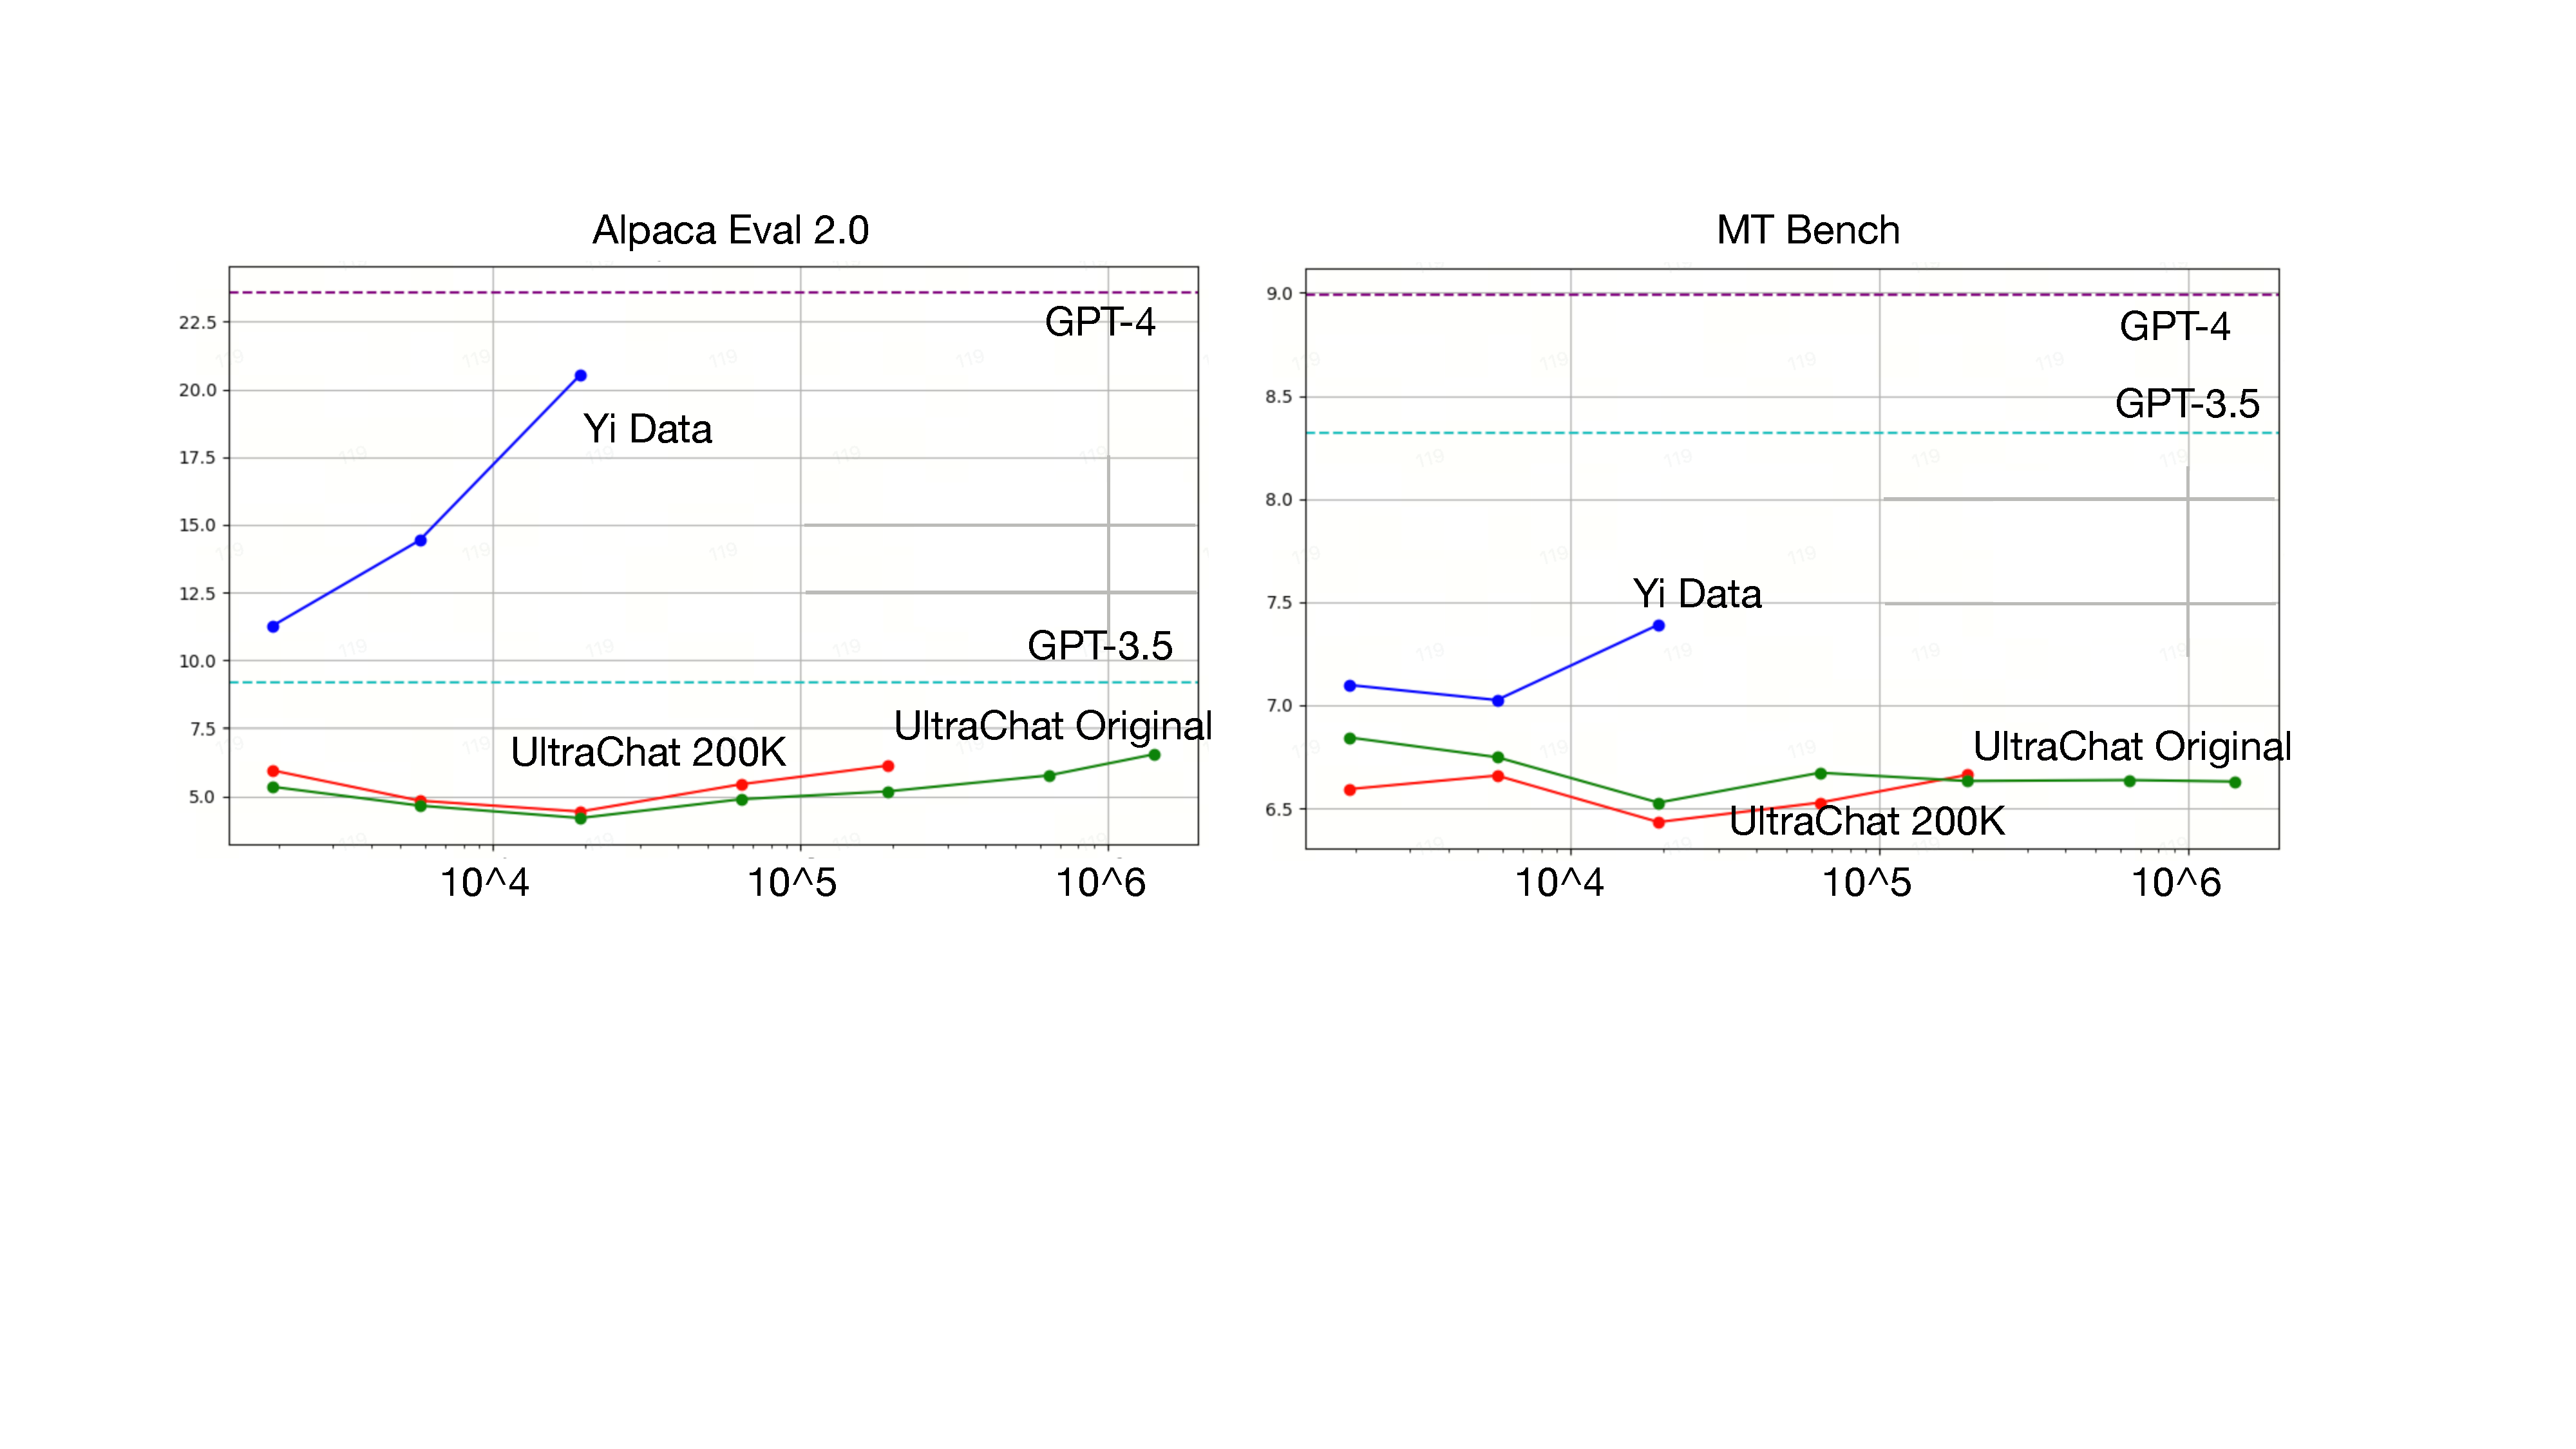
\includegraphics[width=\textwidth]{images/sftdata.pdf}
	\end{center}
	\caption{SFT data scaling curve. Compared with UltraChat and its cleaned version UltraChat 200K, our SFT data demonstrates clear scaling advantages. We attribute its steep slope to the data quality. 
        } %
	\label{fig:sftdata}
\end{figure}
We further demonstrate the data quality by comparing the speed of preference increase during data scaling.
As is shown in Fig.~\ref{fig:sftdata}, when compared with UltraChat~\citep{ding2023enhancing} and its cleaned version UltraChat 200K, we see a clear tendency of performance improvements when scaling up the Yi data. 